\documentclass[]{article}
\usepackage{lmodern}
\usepackage{amssymb,amsmath}
\usepackage{ifxetex,ifluatex}
\usepackage{fixltx2e} % provides \textsubscript
\usepackage{subfig}
\ifnum 0\ifxetex 1\fi\ifluatex 1\fi=0 % if pdftex
  \usepackage[T1]{fontenc}
  \usepackage[utf8]{inputenc}
\else % if luatex or xelatex
  \ifxetex
    \usepackage{mathspec}
  \else
    \usepackage{fontspec}
  \fi
  \defaultfontfeatures{Ligatures=TeX,Scale=MatchLowercase}
\fi
% use upquote if available, for straight quotes in verbatim environments
\IfFileExists{upquote.sty}{\usepackage{upquote}}{}
% use microtype if available
\IfFileExists{microtype.sty}{%
\usepackage[]{microtype}
\UseMicrotypeSet[protrusion]{basicmath} % disable protrusion for tt fonts
}{}
\PassOptionsToPackage{hyphens}{url} % url is loaded by hyperref
\usepackage[unicode=true]{hyperref}
\hypersetup{
            pdfborder={0 0 0},
            breaklinks=true}
\urlstyle{same}  % don't use monospace font for urls
\usepackage[margin=2cm]{geometry}
\usepackage{color}
\usepackage{fancyvrb}
\newcommand{\VerbBar}{|}
\newcommand{\VERB}{\Verb[commandchars=\\\{\}]}
\DefineVerbatimEnvironment{Highlighting}{Verbatim}{commandchars=\\\{\}}
% Add ',fontsize=\small' for more characters per line
\newenvironment{Shaded}{}{}
\newcommand{\KeywordTok}[1]{\textcolor[rgb]{0.00,0.44,0.13}{\textbf{#1}}}
\newcommand{\DataTypeTok}[1]{\textcolor[rgb]{0.56,0.13,0.00}{#1}}
\newcommand{\DecValTok}[1]{\textcolor[rgb]{0.25,0.63,0.44}{#1}}
\newcommand{\BaseNTok}[1]{\textcolor[rgb]{0.25,0.63,0.44}{#1}}
\newcommand{\FloatTok}[1]{\textcolor[rgb]{0.25,0.63,0.44}{#1}}
\newcommand{\ConstantTok}[1]{\textcolor[rgb]{0.53,0.00,0.00}{#1}}
\newcommand{\CharTok}[1]{\textcolor[rgb]{0.25,0.44,0.63}{#1}}
\newcommand{\SpecialCharTok}[1]{\textcolor[rgb]{0.25,0.44,0.63}{#1}}
\newcommand{\StringTok}[1]{\textcolor[rgb]{0.25,0.44,0.63}{#1}}
\newcommand{\VerbatimStringTok}[1]{\textcolor[rgb]{0.25,0.44,0.63}{#1}}
\newcommand{\SpecialStringTok}[1]{\textcolor[rgb]{0.73,0.40,0.53}{#1}}
\newcommand{\ImportTok}[1]{#1}
\newcommand{\CommentTok}[1]{\textcolor[rgb]{0.38,0.63,0.69}{\textit{#1}}}
\newcommand{\DocumentationTok}[1]{\textcolor[rgb]{0.73,0.13,0.13}{\textit{#1}}}
\newcommand{\AnnotationTok}[1]{\textcolor[rgb]{0.38,0.63,0.69}{\textbf{\textit{#1}}}}
\newcommand{\CommentVarTok}[1]{\textcolor[rgb]{0.38,0.63,0.69}{\textbf{\textit{#1}}}}
\newcommand{\OtherTok}[1]{\textcolor[rgb]{0.00,0.44,0.13}{#1}}
\newcommand{\FunctionTok}[1]{\textcolor[rgb]{0.02,0.16,0.49}{#1}}
\newcommand{\VariableTok}[1]{\textcolor[rgb]{0.10,0.09,0.49}{#1}}
\newcommand{\ControlFlowTok}[1]{\textcolor[rgb]{0.00,0.44,0.13}{\textbf{#1}}}
\newcommand{\OperatorTok}[1]{\textcolor[rgb]{0.40,0.40,0.40}{#1}}
\newcommand{\BuiltInTok}[1]{#1}
\newcommand{\ExtensionTok}[1]{#1}
\newcommand{\PreprocessorTok}[1]{\textcolor[rgb]{0.74,0.48,0.00}{#1}}
\newcommand{\AttributeTok}[1]{\textcolor[rgb]{0.49,0.56,0.16}{#1}}
\newcommand{\RegionMarkerTok}[1]{#1}
\newcommand{\InformationTok}[1]{\textcolor[rgb]{0.38,0.63,0.69}{\textbf{\textit{#1}}}}
\newcommand{\WarningTok}[1]{\textcolor[rgb]{0.38,0.63,0.69}{\textbf{\textit{#1}}}}
\newcommand{\AlertTok}[1]{\textcolor[rgb]{1.00,0.00,0.00}{\textbf{#1}}}
\newcommand{\ErrorTok}[1]{\textcolor[rgb]{1.00,0.00,0.00}{\textbf{#1}}}
\newcommand{\NormalTok}[1]{#1}
\usepackage{graphicx,grffile}
\makeatletter
\def\maxwidth{\ifdim\Gin@nat@width>\linewidth\linewidth\else\Gin@nat@width\fi}
\def\maxheight{\ifdim\Gin@nat@height>\textheight\textheight\else\Gin@nat@height\fi}
\makeatother
% Scale images if necessary, so that they will not overflow the page
% margins by default, and it is still possible to overwrite the defaults
% using explicit options in \includegraphics[width, height, ...]{}
\setkeys{Gin}{width=\maxwidth,height=\maxheight,keepaspectratio}
\IfFileExists{parskip.sty}{%
\usepackage{parskip}
}{% else
\setlength{\parindent}{0pt}
\setlength{\parskip}{6pt plus 2pt minus 1pt}
}
\setlength{\emergencystretch}{3em}  % prevent overfull lines
\providecommand{\tightlist}{%
  \setlength{\itemsep}{0pt}\setlength{\parskip}{0pt}}
\setcounter{secnumdepth}{0}
% Redefines (sub)paragraphs to behave more like sections
\ifx\paragraph\undefined\else
\let\oldparagraph\paragraph
\renewcommand{\paragraph}[1]{\oldparagraph{#1}\mbox{}}
\fi
\ifx\subparagraph\undefined\else
\let\oldsubparagraph\subparagraph
\renewcommand{\subparagraph}[1]{\oldsubparagraph{#1}\mbox{}}
\fi

% set default figure placement to htbp
\makeatletter
\def\fps@figure{htbp}
\makeatother


\date{}

\begin{document}

\section{CMPUT 659 Assignment 1
Report}\label{cmput-659-assignment-1-report}

\href{https://github.com/uduse/cmput-659-xai}{-\textgreater{} github}

\subsection{The Domain Specific Language
(DSL)}\label{the-domain-specific-language-dsl}

The provided DSL is very limited in flexibility and parsing string
representation of a DSL is convoluted. As a result, I wrote my own
version of the DSL.

\subsubsection{DSL Grammar}\label{dsl-grammar}

\begin{Shaded}
\begin{Highlighting}[]
\NormalTok{grammar }\OperatorTok{=}\NormalTok{ \{}
\NormalTok{    Rule.START: (}
\NormalTok{        Rule.BLOCK,}
\NormalTok{    ),}
\NormalTok{    Rule.BLOCK: (}
        \CommentTok{# this sampler allows repeating if blocks}
        \CommentTok{# the probability of the second if block appears is 0.6}
        \CommentTok{# the probability of the third if block appears is 0.6 * 0.6 = 0.36, etc.}
\NormalTok{        Diminishing(}\FloatTok{0.6}\NormalTok{, Rule.IF_BLOCK),}
\NormalTok{    ),}
\NormalTok{    Rule.IF_BLOCK: (}
\NormalTok{        [Rule.BOOL_EXP, Rule.IF_BODY],}
\NormalTok{    ),}
\NormalTok{    Rule.IF_BODY: [}
        \CommentTok{# This sampler allows weighted random choice}
        \CommentTok{# here, a return will be chosen 70% of the time,}
        \CommentTok{# while an extra block appears at 30% of the time}
\NormalTok{        Weighted(\{}
            \DecValTok{7}\NormalTok{: Rule.RETURN,}
            \DecValTok{3}\NormalTok{: [Rule.BLOCK, Rule.RETURN],}
\NormalTok{        \})}
\NormalTok{    ],}
\NormalTok{    Rule.BOOL_EXP: [}
\NormalTok{        Rule.BOOL, }
\NormalTok{        Rule.AND_EXP,}
\NormalTok{        Rule.NOT_EXP,}
\NormalTok{    ],}
\NormalTok{    Rule.AND_EXP: (}
\NormalTok{        [Rule.BOOL, Rule.BOOL],}
\NormalTok{    ),}
\NormalTok{    Rule.NOT_EXP: (}
\NormalTok{        Rule.BOOL,}
\NormalTok{    ),}
\NormalTok{    Rule.BOOL: (}
\NormalTok{        Rule.FUNC_CALL,}
\NormalTok{    ),}
\NormalTok{    Rule.FUNC_CALL: }\BuiltInTok{tuple}\NormalTok{(}
        \CommentTok{# here we parse all the library functions into rules}
\NormalTok{        make_dynamic_rule(name) }\ControlFlowTok{for}\NormalTok{ name }\KeywordTok{in}\NormalTok{ lib_func_names}
\NormalTok{    ),}
\NormalTok{    Rule.RETURN: (}
        \StringTok{"return a"}\NormalTok{,}
\NormalTok{    ),}
\NormalTok{    Rule.COLUMN_NUM: (}
        \StringTok{'2'}\NormalTok{, }\StringTok{'3'}\NormalTok{, }\StringTok{'4'}\NormalTok{, }\StringTok{'5'}\NormalTok{, }\StringTok{'6'}
\NormalTok{    ),}
\NormalTok{    Rule.SMALL_NUM: (}
        \StringTok{'0'}\NormalTok{, }\StringTok{'1'}\NormalTok{, }\StringTok{'2'}
\NormalTok{    )}
\NormalTok{\}}
\end{Highlighting}
\end{Shaded}

\subsubsection{DSL Representation}\label{dsl-representation}

The grammar defines the space of Abstract Syntax Tree (AST).

Here's an example of an AST in the space.

\begin{verbatim}
Rule.START
+-- Rule.BLOCK
    +-- Rule.IF_BLOCK
        |-- Rule.BOOL_EXP
        |   +-- Rule.AND_EXP
        |       |-- Rule.BOOL
        |       |   +-- Rule.FUNC_CALL
        |       |       |-- Lib.progression_greater_than
        |       |       |-- state
        |       |       +-- Rule.SMALL_NUM
        |       |           +-- 0
        |       +-- Rule.BOOL
        |           +-- Rule.FUNC_CALL
        |               |-- Lib.is_doubles
        |               +-- a
        +-- Rule.IF_BODY
            +-- Rule.RETURN
                +-- return a
\end{verbatim}

\subsubsection{Script Generation}\label{script-generation}

A script is generated by rendering its corresponding AST. The process of
sampling an AST from the grammar is stochastic, while rendering an AST
to a script is deterministic.

Here's the script obtained by rendering the above AST:

\begin{Shaded}
\begin{Highlighting}[]
\KeywordTok{class}\NormalTok{ Script_7534b62840e04041a875ae6799b31c31(Script):}
    \KeywordTok{def}\NormalTok{ get_action(}\VariableTok{self}\NormalTok{, state):}
\NormalTok{        actions }\OperatorTok{=}\NormalTok{ state.available_moves()}
        \ControlFlowTok{for}\NormalTok{ a }\KeywordTok{in}\NormalTok{ actions:}
            \ControlFlowTok{if}\NormalTok{ (}\KeywordTok{not}\NormalTok{ (Lib.progression_greater_than(}\VariableTok{self}\NormalTok{, }\StringTok{"5f73ea86"}\NormalTok{, state, }\DecValTok{0}\NormalTok{))}
                \KeywordTok{and}\NormalTok{ (Lib.is_doubles(a))):}
                \ControlFlowTok{return}\NormalTok{ a}
            \ControlFlowTok{pass}
        \ControlFlowTok{return}\NormalTok{ actions[}\DecValTok{0}\NormalTok{]}
\end{Highlighting}
\end{Shaded}

\subsection{My Script}\label{my-script}

I wrote my script in a way that the grammar can actually generates it. I
will describe my intentions with the comments inside of the code:

\begin{Shaded}
\begin{Highlighting}[]
\KeywordTok{class}\NormalTok{ MyScript(Script):}
    \KeywordTok{def}\NormalTok{ get_action(}\VariableTok{self}\NormalTok{, state):}
\NormalTok{        actions }\OperatorTok{=}\NormalTok{ state.available_moves()}
        \ControlFlowTok{for}\NormalTok{ a }\KeywordTok{in}\NormalTok{ actions:}
            \CommentTok{# I want to first differentiate between 'yes' and 'no' actions}
            \ControlFlowTok{if}\NormalTok{ (Lib.is_no_action(}\VariableTok{self}\NormalTok{, }\StringTok{""}\NormalTok{, a)):}
                \CommentTok{# If it's a 'no', then we select it when we finished a column this round}
                \ControlFlowTok{if}\NormalTok{ (Lib.has_won_column(}\VariableTok{self}\NormalTok{, }\StringTok{""}\NormalTok{, state, a)):}
                    \ControlFlowTok{return}\NormalTok{ a}
                
            \ControlFlowTok{if}\NormalTok{ (Lib.is_yes_action(}\VariableTok{self}\NormalTok{, }\StringTok{""}\NormalTok{, a)):}
                \CommentTok{# if it's a 'yes', then we select it when we made too little progress this game}
                \ControlFlowTok{if}\NormalTok{ (}\KeywordTok{not}\NormalTok{ Lib.progression_greater_than(}\VariableTok{self}\NormalTok{, }\StringTok{""}\NormalTok{, state, }\DecValTok{2}\NormalTok{)}
                   \KeywordTok{and} \KeywordTok{not}\NormalTok{ Lib.has_won_column(}\VariableTok{self}\NormalTok{, }\StringTok{""}\NormalTok{, state, a)):}
                    \ControlFlowTok{return}\NormalTok{ a}
                \CommentTok{# or if we made too little progress this round}
                \ControlFlowTok{if}\NormalTok{ (}\KeywordTok{not}\NormalTok{ (Lib.progression_this_round_greater_than(}\VariableTok{self}\NormalTok{, }\StringTok{""}\NormalTok{, state, }\DecValTok{1}\NormalTok{))):}
                    \ControlFlowTok{return}\NormalTok{ a}

            \CommentTok{# we prioritize actions that win a column for us}
            \ControlFlowTok{if}\NormalTok{ (Lib.action_wins_column(}\VariableTok{self}\NormalTok{, }\StringTok{""}\NormalTok{, state, a)):}
                \ControlFlowTok{return}\NormalTok{ a}
                
            \CommentTok{# also always choose a double if we have a chance}
            \ControlFlowTok{if}\NormalTok{ (Lib.is_doubles(}\VariableTok{self}\NormalTok{, }\StringTok{""}\NormalTok{, a)):}
                \ControlFlowTok{return}\NormalTok{ a}
               
        \ControlFlowTok{return}\NormalTok{ actions[}\DecValTok{0}\NormalTok{]}
\end{Highlighting}
\end{Shaded}

This script has a win rate of 0.93 against the random agent, which I
think is pretty good. I also evaluated this script against the best
script generated by the genetic algorithm, and it still has a win rate
of 0.45, which is still decent.

\subsection{Redundancy Removal}\label{redundancy-removal}

My grammar supports \texttt{not} and \texttt{and} operation and that
makes function calls that always returns \texttt{False} still
meaningful. This means any function that has been called at least once
during the evaluation is meaningful to the script. To move redundancy in
the scripts, first we need to record what functions are actually called.

I achieved this by these following steps:

\paragraph{1. bind functions to AST
nodes}\label{bind-functions-to-ast-nodes}

By binding functions to their corresponding AST nodes, we are able to
map script content back to specific nodes in the AST. This is done by
assigning ID to AST nodes, and have all functions rendered in a way that
incorporates the ID. For example, in the above script, we have a
function like:

\begin{Shaded}
\begin{Highlighting}[]
\NormalTok{Lib.action_wins_column(}\VariableTok{self}\NormalTok{, }\StringTok{"5f73ea86"}\NormalTok{, state, a)}
\end{Highlighting}
\end{Shaded}

The second argument \texttt{"5f73ea86"} is the ID of the corresponding
node in the AST. Once this function is called, it will have a side
effect of adding itself to the \texttt{set} of all IDs of called
functions, stored in \texttt{self.call\_log}. In other words, once the
above function is called, \texttt{self.call\_log} will contain
\texttt{"5f73ea86"} which means the node \texttt{"5f73ea86"} is marked
as ``called''.

Now, we can remove unused function calls by pruning the AST based on the
\texttt{call\_log}. However, this requires some fixing to the AST as
simply taking away functions that are not called could break the
validity of the AST.

For example, in \texttt{func1()\ and\ func2()}, if \texttt{func1()}
always returns \texttt{True}, \texttt{func2} will never be called. If we
want to remove \texttt{func2()}, we would need to change the AST so
\texttt{func1()} is no longer a part of a \texttt{Rule.AND} . There are
many other ways that removing a function call would break the AST.

As a result, we want to remove in-effective blocks instead, since blocks
can be removed without breaking the AST.

\paragraph{2. bubble up marks}\label{bubble-up-marks}

How do we decide what block is effective? We say that a block is
effective when at least one of its children is effective. Therefore, we
want to update the \texttt{call\_log} so it includes all nodes that have
at least one marked child. We achieve this by bubbling the marks for all
nodes in the \texttt{call\_log}.

For example, if we have an AST with marked nodes denoted as \texttt{X}:

\begin{verbatim}
O
+-- O
    +-- X
    +-- O
\end{verbatim}

We bubble up the marks and now it will look like this:

\begin{verbatim}
X
+-- X
    +-- X
    +-- O
\end{verbatim}

\paragraph{3. remove nodes in the AST}\label{remove-nodes-in-the-ast}

Now we know that all nodes that are not marked have no impact during the
evaluation. We remove all these nodes. In the case of the tree above, we
will have:

\begin{verbatim}
X
+-- X
    +-- X
\end{verbatim}

If we removed any of the nodes, the script has to be re-rendered based
on the new AST.

\subsection{Genetic Algorithm}\label{genetic-algorithm}

\subsubsection{Mutation}\label{mutation}

Since I render scripts based on ASTs, mutations can be managed in a more
fine-grained way by replacing subtrees. This means mutations can happen
in any level of the grammar, from replacing the whole script to changing
a specific parameter in a function call.

To mutate a script, we first first choose a node randomly from its AST.
Then, that node is removed from the AST and a new subtree is built base
on the type of the removed node using the same grammar.

\subsubsection{Crossover}\label{crossover}

To crossover to script, we first randomly choose one
\texttt{Rule.IF\_BLOCK} from both of them as subtree heads. Then, we
swap the subtrees of these two ASTs and render new scripts based on the
new ASTs.

\subsection{Results}\label{results}

I would like to see how these factors in my genetic algorithm affects
the result:

\begin{itemize}
\tightlist
\item
  population size
\item
  number of games for evaluation
\item
  number of elites to keep for each generation
\end{itemize}

I will do this comparison by keeping the other parameters the same while
adjusting the target parameter.

\begin{figure}[h]%
  \centering
  \subfloat[population = 8]{{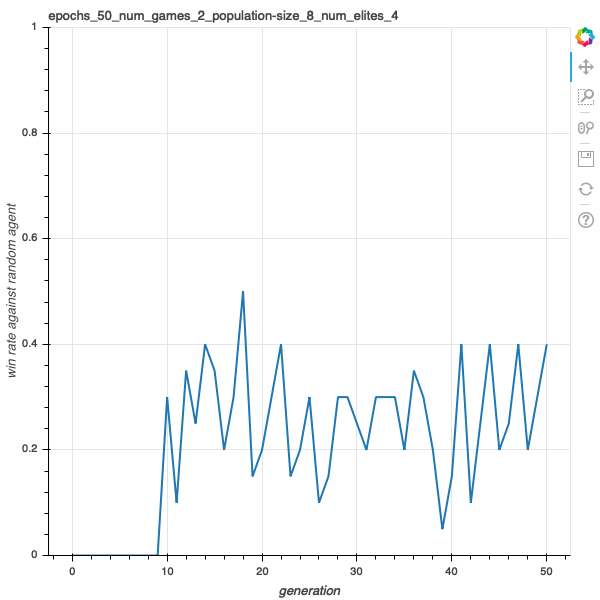
\includegraphics[width=5cm]{results/epochs_50_num_games_2_population-size_8_num_elites_4.png} }}%
  \qquad
  \subfloat[population = 12]{{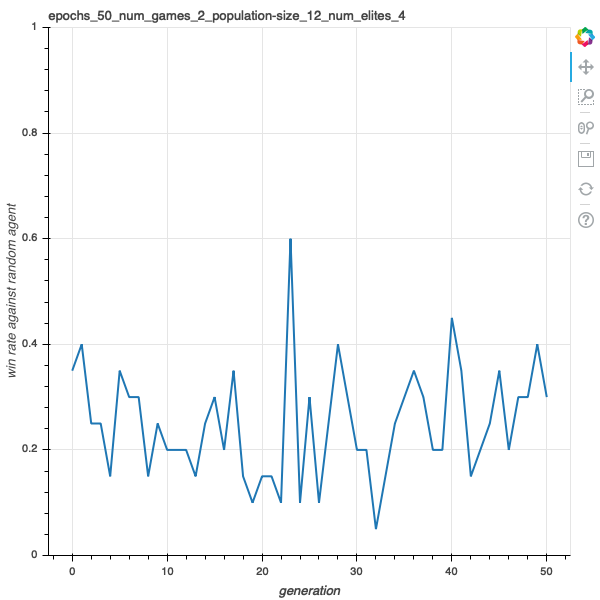
\includegraphics[width=5cm]{results/epochs_50_num_games_2_population-size_12_num_elites_4.png} }}%
  \qquad
  \subfloat[population = 16]{{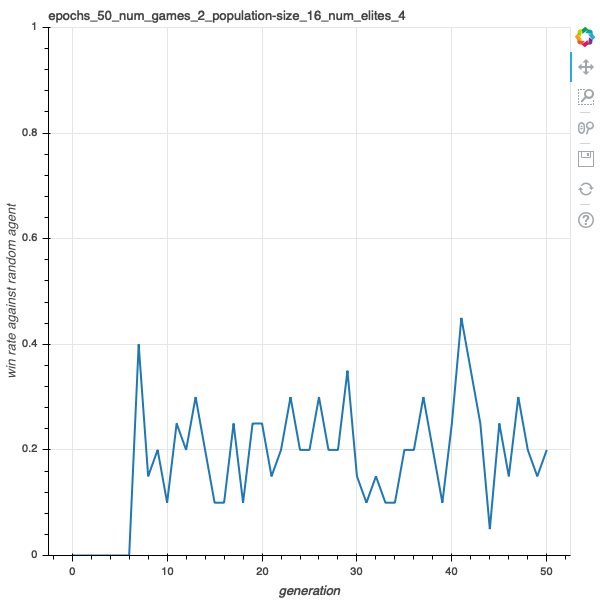
\includegraphics[width=5cm]{results/epochs_50_num_games_2_population-size_16_num_elites_4.png} }}%
  \qquad
  \subfloat[population = 20]{{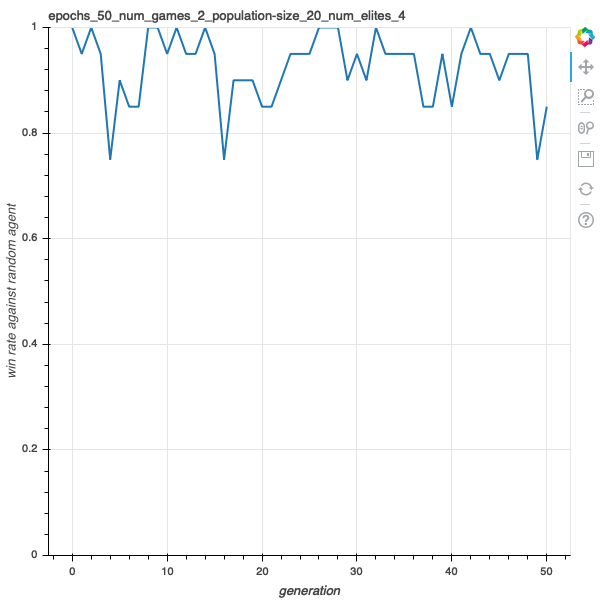
\includegraphics[width=5cm]{results/epochs_50_num_games_2_population-size_20_num_elites_4.png} }}%
  \caption{Changing Population Size}%
  \label{fig:example}%
\end{figure}

\begin{figure}[h]%
  \centering
  \subfloat[number of games = 1]{{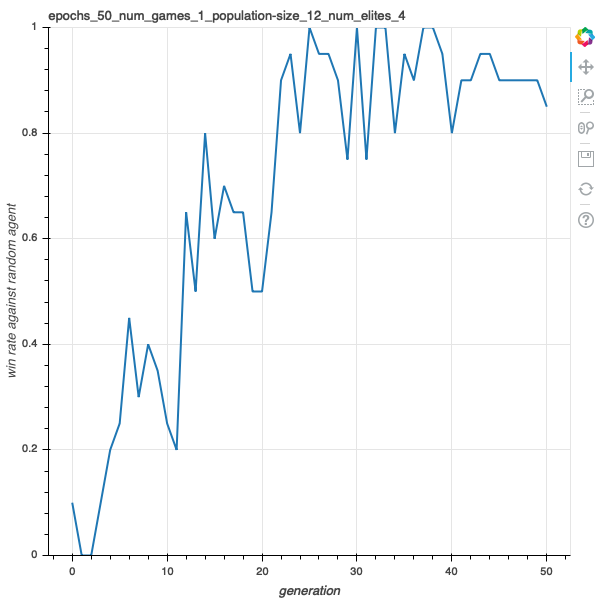
\includegraphics[width=5cm]{results/epochs_50_num_games_1_population-size_12_num_elites_4.png} }}%
  \qquad
  \subfloat[number of games = 2]{{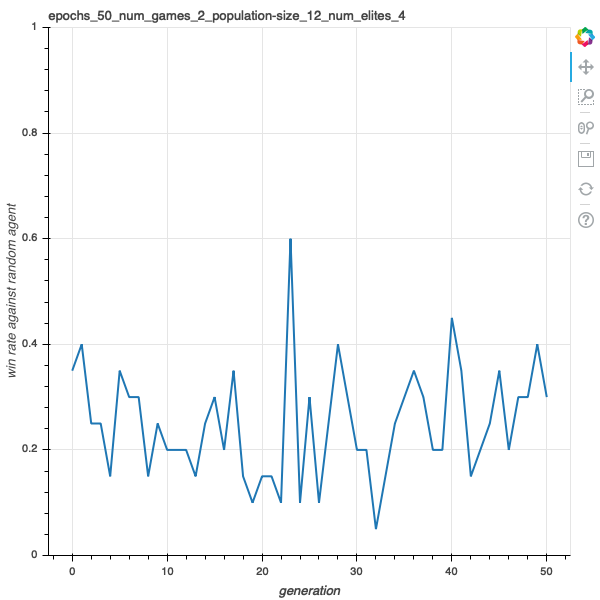
\includegraphics[width=5cm]{results/epochs_50_num_games_2_population-size_12_num_elites_4.png} }}%
  \qquad
  \subfloat[number of games = 3]{{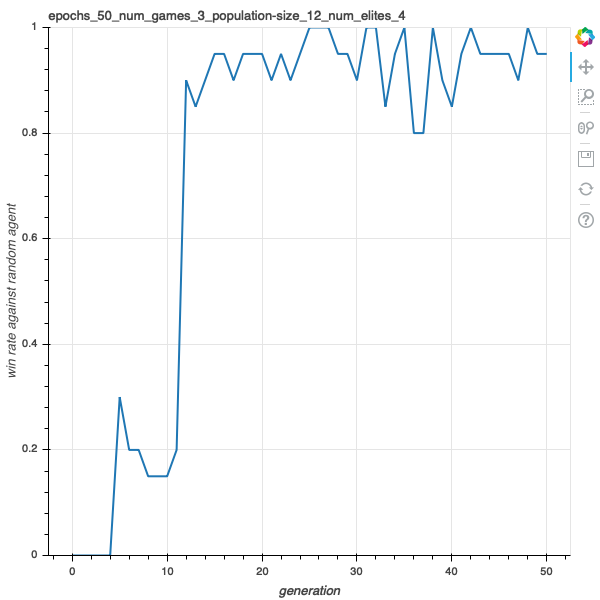
\includegraphics[width=5cm]{results/epochs_50_num_games_3_population-size_12_num_elites_4.png} }}%
  \caption{Changing Number of Games Played}%
  \label{fig:example}%
\end{figure}

\begin{figure}[h]%
  \centering
  \subfloat[number of elites = 1]{{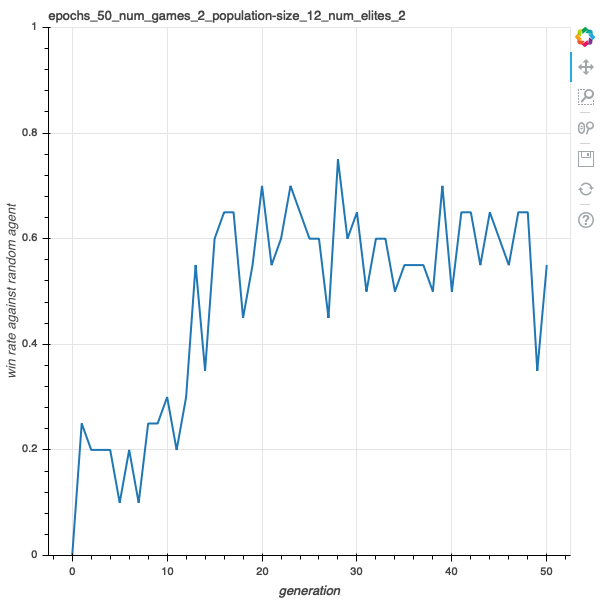
\includegraphics[width=5cm]{results/epochs_50_num_games_2_population-size_12_num_elites_2.png} }}%
  \qquad
  \subfloat[number of elites = 2]{{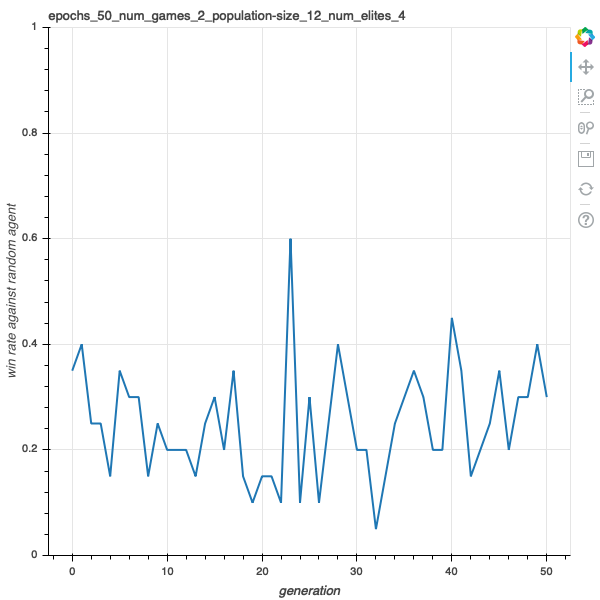
\includegraphics[width=5cm]{results/epochs_50_num_games_2_population-size_12_num_elites_4.png} }}%
  \qquad
  \subfloat[number of elites = 3]{{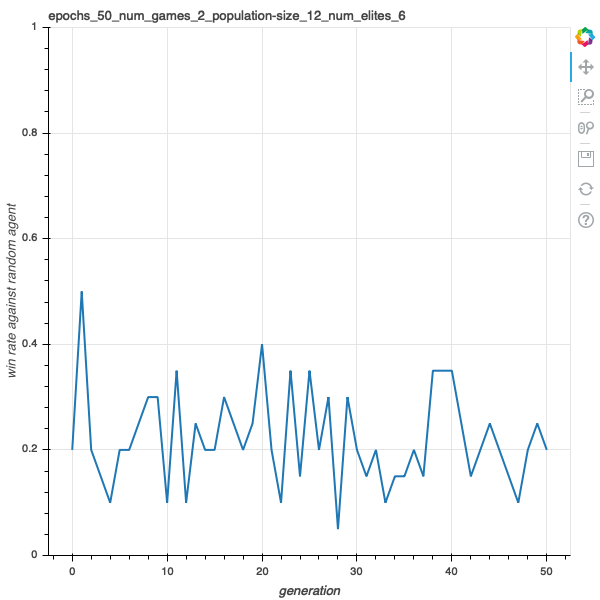
\includegraphics[width=5cm]{results/epochs_50_num_games_2_population-size_12_num_elites_6.png} }}%
  \caption{Changing Number of Elites}%
  \label{fig:example}%
\end{figure}

As we can see, larger population increases the population overall win
rate of the scripts.
It seems that the number of games played has no direct impact on the
quality of the scripts generated.

Aa we can see, having more elites negatively impacts the quality of the
scripts generated. My guess is that too many elites limits the potential
space for mutation and crossover, so better scripts are less likely to
emerge.

\subsection{Discussion}\label{discussion}

\subsubsection{thoughts on generating scripts with genetic
algorithm}\label{thoughts-on-generating-scripts-with-genetic-algorithm}

I felt that generating scripts with genetic algorithm and training
neural networks are alike. Neural network training techniques are
sometimes referred as ``alchemy'' or ``black magic''. This is because
taking an action, like changing a parameter, leads to undefined
behavior. Though this undefined behavior is somehow correlated to the
action, one may only make guesses based on their experience and common
practices. When one's goal is to improve a specific metric while
influences of different approaches are not obvious, one may only make
best guesses and do experiments with trials and errors. For this
specific assignment, I spent a lot of time experimenting with different
things but still unaware of their real impact on the result.

The things I tried include:

\begin{itemize}
\tightlist
\item
  add more library functions for scripts to utilize
\item
  use more expressive grammar to allow advanced scripts
\item
  limit mutation rate to allow keeping of good scripts
\item
  limit crossover subtree size to disable huge replacements
\end{itemize}

I failed to isolate variables in experiments and confidently tell the
influence of a specific change to the algorithm. This is mainly due to
the randomness in generating scripts combined with the time cost of
doing experiments. If the outcomes are more arbitrary, then we need to
do more experiments to be confident. However, the time cost of doing
less arbitrary experiments is higher (e.g, using a larger population
size, using more epochs, playing more games during evaluation), and this
conundrum cannot be avoided easily. Consequently, the plots I displayed
in the ``Results'' section are not as convincing since too little
experiments were ran for it.

Maybe hyper-parameter tuning would reduce this problem of adjusting
parameters headlessly, but that requires even more computations.

\subsubsection{comparison between my script and the genetically evolved
script}\label{comparison-between-my-script-and-the-genetically-evolved-script}

I discovered that function \texttt{has\_won\_column} used together with
\texttt{is\_no\_action} significant improves a script's performance.
Even without other clauses these two functions can produce a script that
beats an random agent 90\% of the time. It's not surprising that almost
all of the scripts

\subsubsection{is the smaller version of Can't stop an interesting
game?}\label{is-the-smaller-version-of-cant-stop-an-interesting-game}

Not really. First of all, the game is too simple. There aren't many
decisions you can make during a game. In addition, some rules are way
superior to others, making the genetic algorithm all about find these
superior rules. Secondly, there are too little interactions between
players. The only thing that matters is the control of a specific
column. Other than that, the script just do its own things.

\subsubsection{scripts for the commercial version of Can't
stop}\label{scripts-for-the-commercial-version-of-cant-stop}

My scripts showed there are only a few things you have to think to play
well, and other observations are not very important. This means the game
can be boring once all the players know to stop when they take control
over a column, and the rest are largely decided by luck. Heavily luck
dependent games are not welcomed unless real in-game currency is
involved (i.e.~unless it's gambling). So I would vote against the
development of a commercial version of the game since either it will be
boring or it will involve gambling.

\end{document}
